\newcommand\abs[1]{\ensuremath{\lvert #1 \rvert}}

\subsection{3-Clique merge with insertion}
\label{3clique_merge}
\subsubsection*{Research method}

We will compare the models performance on Planetoid/CORA dataset~\cite{cora_dataset} while classifying nodes of the graph.
The dataset consists of exactly one undirected graph.
The graph represents a citation network --- nodes are scientific papers, and edges are citations (if two nodes are connected then one paper cites the other).

There are 2708 nodes and 10556 edges, and each node has a feature vector of length 1433 which stores the number of occurrences of 1433 predefined words.
Each node (paper) is a member of exactly one of seven classes.

The training node label rate is 5\%, which means that the neural network knows classes of 5\% of nodes while learning.

The benchmark will be performed by taking average of 100 runs of 300 epochs.

\subsubsection*{Description}

In this experiment we find all the 3-cliques~\cite{wiki_clique} (triangles) in the graph, then sort them based on `distance' and replace each 3-clique with one node (called \emph{merged node}) sharing the features of the initial three.

The following figures show exactly how a 3-clique is merged: the resulting feature vector is the average of the feature vectors of initial nodes: $\frac{1}{3} \cdot \left( (1, 4, 5) + (2, 7, 1) + (0, 1, 6) \right) = \frac{1}{3} \cdot (3, 12, 12) = (1, 4, 4)$


\begin{figure}[h]
\centering
\begin{minipage}{.7\textwidth}
  \centering
  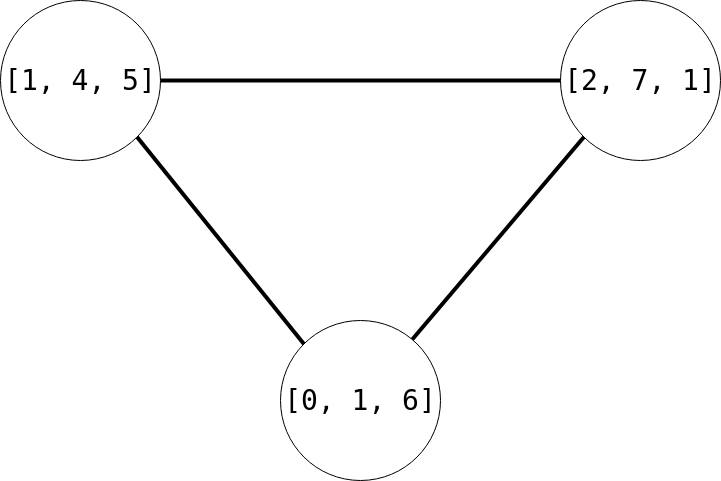
\includegraphics[width=.4\linewidth]{3clique_before_merge_example}
  \captionof{figure}{An example of a 3-clique}
  \label{fig:test1}
\end{minipage}%
\begin{minipage}{.3\textwidth}
  \centering
	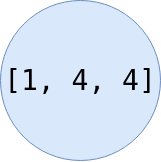
\includegraphics[width=.3\linewidth]{3clique_merged_example}
  \captionof{figure}{Same 3-clique but merged}
  \label{fig:test2}
\end{minipage}
\end{figure}

The source code is available in the project repository and can be found in the `experiments' directory~\cite{3clique_ins_experiment}.

\subsubsection*{Algorithm}

Firstly, let us define a 3-clique more formally.
We define it as follows: $
	\{ \left(a, b, c\right)\
	\lvert\ a, b, c \in V \wedge
	\left(a, b\right),
	\left(a, c\right),
	\left(b, c\right) \in E \} $.

While merging nodes in the cliques, we might face a problem: some of the nodes might participate in several 3-cliques.
In order to solve it, we need to introduce a mechanism for ordering cliques so that we could show preference to one instead of the other.
Naturally, such a mechanism should rely on the nodes feature vectors.
There are 2 major distance calculating algorithms: Euclidean distance and Manhattan distance.
Since the feature vectors are very sparse, the algorithms give quite close results and there is no need to consider them separately.

Using Euclidean distance we can map each 3-clique into a real number by calculating the sum of pairwise distances: $\abs{a_f - b_f}^2 + \abs{a_f - c_f}^2 + \abs{b_f - c_f}^2$, where $v_f$ stands for node's $v$ feature vector.
The resulting ordering now allows us to choose one 3-clique instead of another, since we know that one has its nodes `closer' to each other.

Therefore, one can simply sort all the 3-cliques in ascending order, merge each 3-clique and filter out all the `later' 3-cliques containing nodes from the current one.
This allows us pick the closest and most valuable nodes in a greedy way while also saving us from using a `new' node in another 3-clique ($(a, b, c) \rightarrow a';\ (a', d, e) \rightarrow a''$ is not allowed, since the graph could collapse).

\begin{enumerate}
	\item Find all the 3-cliques in graph.
	\item Sort them according to the sum of distances between nodes
	\item Merge all `valid' 3-cliques in one node. While doing so, we have to preserve all the edges coming in and out of the triplet. For each clique all the other cliques containing nodes from the current one have to be filtered out, so the `merged' nodes will are not merged with others.
	\item Generate new dataset from the resulting graph.
	\item Pass the generated dataset to model.
\end{enumerate}

The process is shown on Figure~\ref{fig:clique_merged}.

\subsubsection*{Results and interpretation}

A benchmark on the Cora dataset~\cite{cora_dataset} had shown that we are able to remove a total of 21.71\% of nodes (the number reduced from 2708 to 2120) and 56.73\% edges (from 10556 to 4568).
Since the operation of merging of all cliques is fast comparing to the model's learning time, we reduced the latter approximately by 29.5\% (on average, went from 4.171s to 2.939s).
This improvement can be also seen on the loss graph of our models:

Speaking of accuracy, we claim it did not change much.
On average, the accuracy of a default model is 0.803, and the model with 3-cliques merged performs practically same --- the average accuracy is 0.746 (both results were achieved by taking average of 100 runs with 300 epochs).
So, the accuracy dropped by 7\% (0.057 in absolute value), while the speed increase was almost 30\%.

\begin{center}
	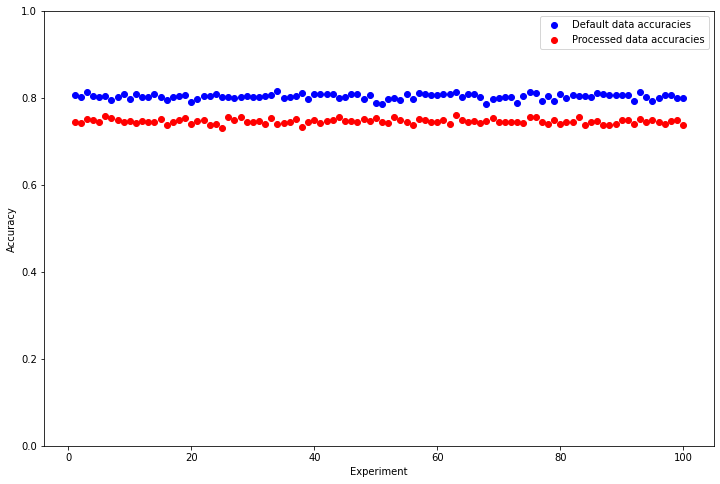
\includegraphics[width=0.75\textwidth]{3clique_accuracy.png}
\end{center}

Therefore, we can claim that the only purpose of merging 3-cliques is reducing the learning time without significant loss of accuracy.
It doesn't make much sense for theoretical purposes, however, is definitely an advantage in production.

\subsection{Infinite 3-clique merge}
\subsubsection*{Description}
In this experiment, the methodology and the algorithm are similar to the `finite 3-clique merge'.
The only difference is that we \emph{allow} merged nodes to participate in merge process again.
The source code is available on GitHub as well~\cite{3clique_inf_merge_experiment}.

\subsubsection*{Results and interpretation}
The proposed method allowed us to remove the majority of information from a graph.
This merge, or convolution, managed to delete as many as 60.12\% of the nodes and 93.79\% of edges.
The performance of learning after this operation increased drastically --- the learning time went from 2.537 seconds to as low as 1.059 seconds (which is only 42\% of the original time).

We can clearly see the improvement on the loss graph below.
We estimate the greatest improvement to be at around 160 epochs, not 300 as we benchmarked.

\begin{figure}[h]
	\centering
	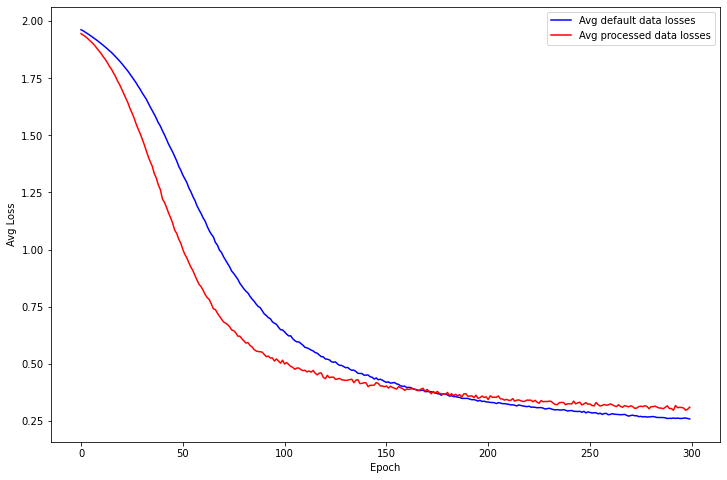
\includegraphics[width=0.7\textwidth]{3clique_inf_loss}
	\caption{Average loss for `default' and processed data}
\end{figure}

However, this comes at a high cost of decreased accuracy.
Average accuracy went from 0.809 to 0.517 which is a 36\% decrease.

\begin{figure}[h]
	\centering
	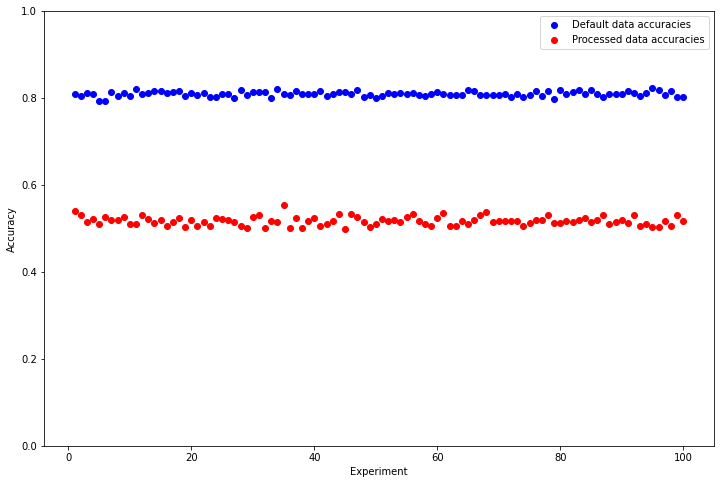
\includegraphics[width=0.7\textwidth]{3clique_inf_accuracy}
	\caption{Accuracies of models with `default' and processed data}
\end{figure}

This extreme graph reduction is probably applicable in some cases, but we think that it would be better to find a balance in the number of number of merges --- heuristically find the number of iterations of algorithm described in Section~\ref{3clique_merge}.

\subsection{Prospects}

In future we want to focus on topological aspect of the transformation presented in the paper.
In particular, we are interested in `infinite merge', where `merged nodes' can be merged again.
We also want to see how the transformation presented can be used in other graph tasks, for example, in graph classification.

Another interesting idea is to exploit other topological feature of a graph.
Sometimes nodes can be weakly connected to each other via edges, while probably having another mean of connections.
For instance, if we consider a map with several coastal cities, we will see that the cities are `chained' (each of them has connections with 2 neighbors) and form some kind of a loop.
We think it is possible to extract information from this form of connection.

